% Tipo de documento y paquetes a utilizar.
\documentclass[12pt]{article}
\usepackage[utf8]{inputenc}
% \usepackage{amsmath, amsthm, amsfonts, mathtools} % Paquete para usar más fórmulas y ecuaciones.
\usepackage{graphicx}       % Paquete para usar imágenes y figuras.
\usepackage{geometry}       % Paquete para trabajar con los márgenes del documento.
\usepackage{fancyhdr}       % Paquete para personalizar encabezado y pie de página.
\usepackage{lastpage}       % Paquete para referenciar páginas del documento.
\usepackage{listings}       % Paquete para escribir código de programación.
\usepackage{inconsolata}    % Paquete de tipo de letra consola.
\usepackage{multirow}       % Paquete para combinar filas y columnas en tablas.
\usepackage{array}          % Paquete para trabajar tablas especializadas.
\usepackage{xcolor}         % Paquete básico para agregar color al texto.
\usepackage{float}          % Paquete para utilizar fijación de figuras H.
\usepackage{hyperref}       % Paquete para insertar links en el documento.
%\usepackage{ragged2e}       % Paquete para cambiar alineación del texto del documento.

% Define colores nuevos
\definecolor{fondo_codigo}{HTML}{E4E4EE}
\definecolor{comentarios_codigo}{HTML}{3C8031}

% Personalización de la fuente para el código.
\lstset{
    %language = CSS,                             % Lenguaje con palabras reservadas de este resaltadas.
    basicstyle = \ttfamily\footnotesize,        % Utiliza la fuente tttfamily, en especial el paquete inconsolata.
    frame = single,                             % Quita el marco al cuadro flotante que contiene el código o texto.
    backgroundcolor = \color{fondo_codigo},     % Cambia el color del fondo del marco del código. Utiliza el paquete "xcolor" y define un nuevo color.
    columns = fullflexible,                     % Ajusta el cuadro flotante al tamaño del texto del documento.
    breaklines = true,                          % Ajusta el texto dentro del contenedor.
    inputencoding = utf8,                       % Admite caracteres del código UTF8.
    extendedchars = true,                       % Soporte para caracteres especiales.
    %numbers = left,                            % Agrega número de línea al código (izquierda, sin número y derecha).
    showstringspaces = false,                   % Quita los guiones bajos predeterminados de los espacios en cadenas de texto.
    escapebegin = \obeyspaces,                  % Complemento de la entrada anterior.
    % rulecolor = \color{red},                  % Color del borde del marco del código.
    % numberstyle = \color{red},                % Color de los números en el texto o código.
    % stringstyle = \color{red},                % Color de las cadenas de texto en el texto o código.
    % keywordstyle = \color{red},               % Color de las palabras reservadas en el texto o código.
    % identifierstyle = \color{red},            % Color del texto o código.
    commentstyle = \color{comentarios_codigo},  % Color de los comentarios en el texto o código.
    literate =                                  % Acepta los siguientes caracteres especiales fuera de UTF8.
        {á}{{\'a}}1 {é}{{\'e}}1 {í}{{\'i}}1 {ó}{{\'o}}1 {ú}{{\'u}}1
        {Á}{{\'A}}1 {É}{{\'E}}1 {Í}{{\'I}}1 {Ó}{{\'O}}1 {Ú}{{\'U}}1
        {ñ}{{\~n}}1 {Ñ}{{\~N}}1,
}

% Márgenes del documento.
\newgeometry{
    top=2.5cm,      % Superior.
    bottom=2.5cm,   % Inferior.
    outer=2.5cm,    % Parte exterior.
    inner=2.5cm,    % Parte interior.
}

% Personalización de la cabecera y pie de página.
\pagestyle{fancy}
\fancyhf{}
\rhead{Overleaf}                                            % Texto en esquina superior derecha.
\lhead{Apuntes de Bootstrap}                                % Texto en esquina superior izquierda.
\rfoot{Pagina \thepage \hspace{1pt} de \pageref{LastPage}}  % Texto en esquina inferior derecha (Página n de n).
% Ancho de línea horizontal superior e inferior.
\renewcommand{\headrulewidth}{1pt}
\renewcommand{\footrulewidth}{1pt}

% Datos para la portada del documento.
\title{Apuntes de Bootstrap}
\author{migueluisV}
\date{Realizadas: Mayo 2023}

% Inicio del documento.
\begin{document}

% Cambia los títulos de los índices:
% Content - Índice
% List of Figures - Índice de Figuras
% List of Tables - Índice de Tablas
\renewcommand*\contentsname{Índice}
\renewcommand{\listtablename}{Índice de Tablas}
\renewcommand{\listfigurename}{Índice de Figuras}

% Inserta la portada y los índices.
\maketitle\newpage
\tableofcontents\newpage
\listoffigures\newpage
\listoftables\newpage

\hspace{0.55cm}Este documento se hizo con \href{https://es.overleaf.com/}{\textbf{Overleaf}} y los ejemplos fueron desarrollados y probados con \textbf{Visual Studio Code}, con su extensión \textbf{Live Server} en el buscador \textbf{Microsoft Edge} o \textbf{Brave}.

\sloppy La estructura HTML de los ejemplos en este documento serán omitidos, dejando únicamente lo vital para que los ejemplos funcionen y para evitar que este trabajo sea muy largo, los ejemplos CSS y Bootstrap si vendrán completos.

% Incluye los archivos que conforman al proyecto.
% https://www.youtube.com/watch?v=QCw0L6FupQ0

\section{Conceptos básicos}

\textbf{Bootstrap}

Se trata de un \textit{framework} de CSS para crear sitios y páginas web \textit{responsivos}.

\textbf{Framework y Framework CSS}

Un Framework es una base o plataforma de un cierto lenguaje de programación para ahorrar a otros desarrolladores el escribir código. Estos frameworks suelen tener contenido, módulos, clases o funciones que resuelven problemas comunes, proporcionando este código para que, quien utilice el framework, tarde menos en desarrollar una implementación.

Un framework CSS es una base con \textit{clases}, \textit{identificadores} y estilos predeterminados que permiten crear páginas web bien distribuidas y responsivas para los distintos tamaños de pantalla disponibles.

\textbf{Páginas y sitios web \textit{responsivos}}

La palabra responsivo viene de la palabra en inglés \textit{responsive}, estas página o sitios web pueden ser llamados también adaptables. Estas páginas son responsivas cuando el tamaño y distribución de la página se adapta a la pantalla del dispositivo que la visualiza, siendo una tableta, celular o computadora.



\section{Agregando Boostrap a un proyecto web}

Esta herramienta no necesita de una instalación en particular, simplemente agregamos una etiqueta al \textit{head} de nuestro proyecto de la siguiente manera:
\begin{lstlisting}
    <!DOCTYPE html>
    <html lang='es'>
        <head>
            <!-- Bootstrap. -->
            <link href="https://cdn.jsdelivr.net/npm/bootstrap@5.3.0-alpha3/dist/css/bootstrap.min.css" rel="stylesheet" integrity="sha384-KK94CHFLLe+nY2dmCWGMq91rCGa5gtU4mk92HdvYe+M/SXH301p5ILy+dN9+nJOZ" crossorigin="anonymous">
            <script src="https://cdn.jsdelivr.net/npm/bootstrap@5.3.0-alpha3/dist/js/bootstrap.bundle.min.js" integrity="sha384-ENjdO4Dr2bkBIFxQpeoTz1HIcje39Wm4jDKdf19U8gI4ddQ3GYNS7NTKfAdVQSZe" crossorigin="anonymous"></script>
        </head>
        <body>
            <!-- Contenido. -->
        </body>
    </html>
\end{lstlisting}

Se agrega las etiquetas \textit{link} y \textit{script} a la cabecera de nuestro proyecto, estas líneas fueron obtenidas de la \href{https://getbootstrap.com/docs/5.3/getting-started/download/#cdn-via-jsdelivr}{\textcolor{cyan}{documentación oficial}} de Boostrap, en la sección de Download en la sección \textbf{CND via jsDelivr}. Debe fijarse bien qué versión va a estar implementando a su proyecto, en nuestro caso es la versión 5.3, puede revisar qué versión tomará en la esquina superior derecha de la página, como se ve en la Figura \ref{fig:1}.
\begin{figure}[H]
    \centering
    \caption{Versión de Bootstrap para agregarlo a un proyecto web}
    \label{fig:1}
    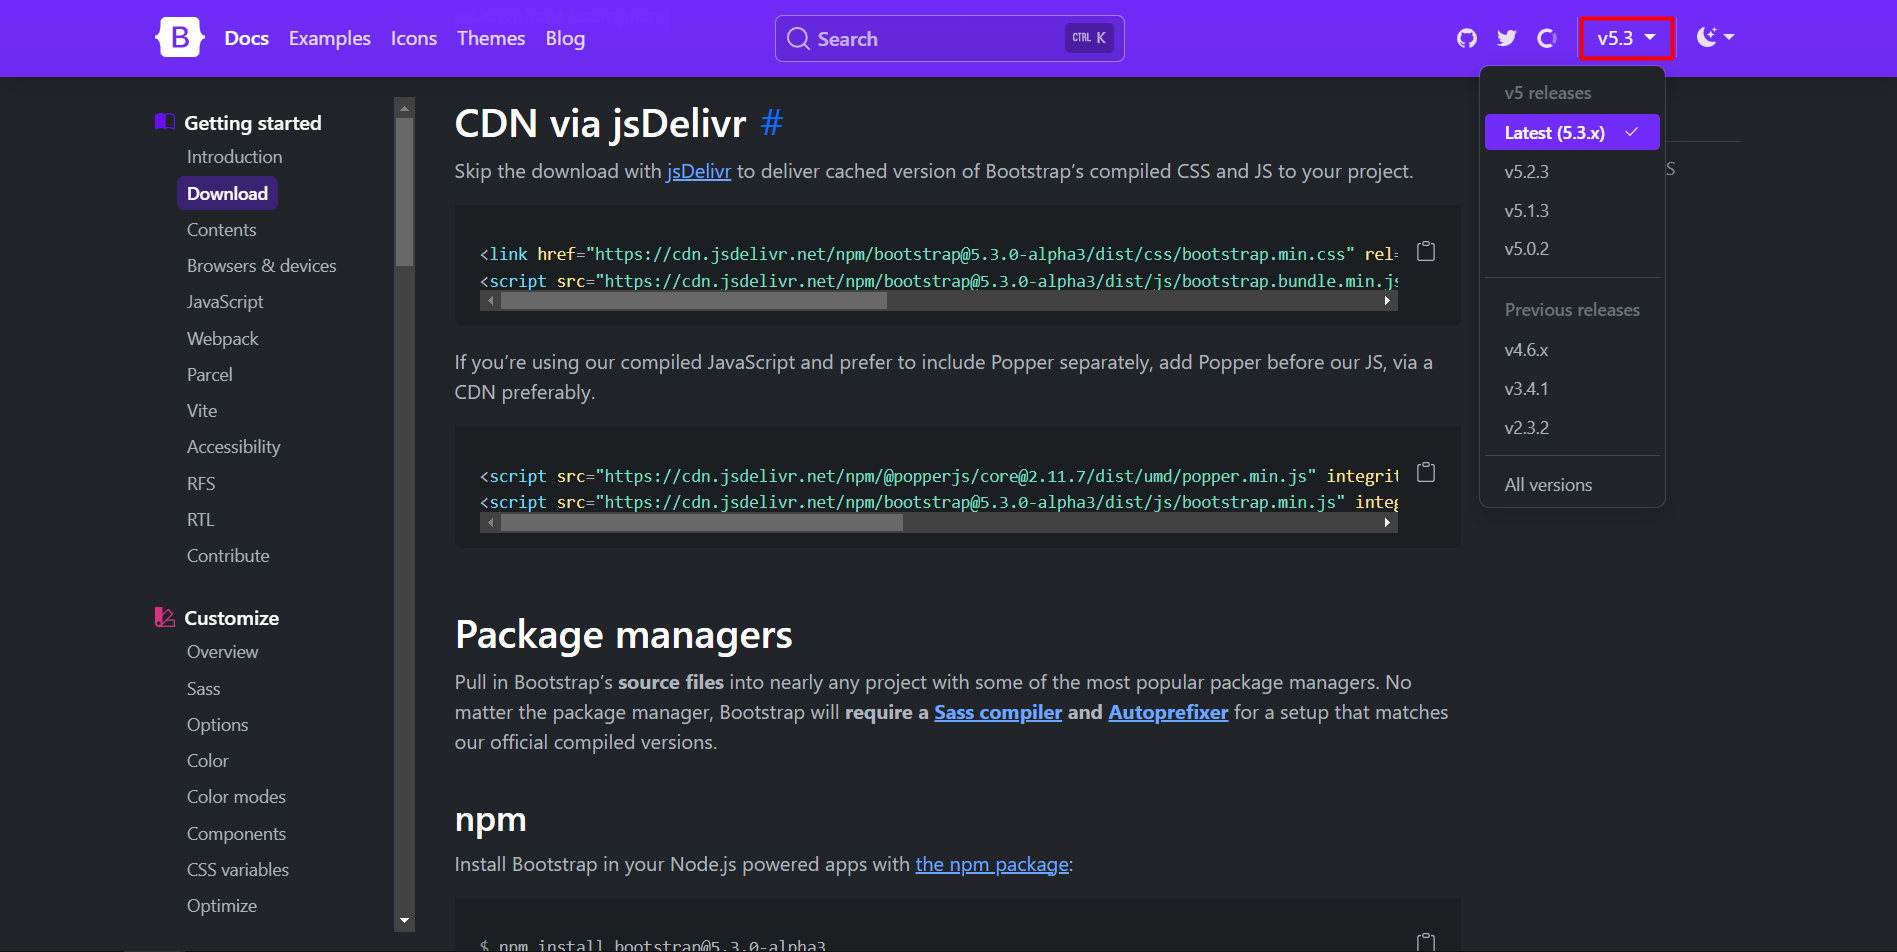
\includegraphics[width=\textwidth]{ss/version-bootstrap.png}
\end{figure}



\section{Los pilares de Bootstrap}


\subsection{Grid}

La Grid (\textit{cuadrícula} en español) define como se estructura los elementos de una página y como se adaptan a un tamaño de pantalla. El Grid se puede definir también como un conjunto de filas, columnas y contenedores que definen como se van a presentar y alinear los elementos de una página web.

Una fila del Grid se divide en 12 secciones o columnas, un elemento HTML o elemento Bootstrap puede abarcar la cantidad de secciones que este requiera, pudiendo ser 3, 5, 7 o las 12 en total, como se ve en la Figura \ref{fig:2} y \ref{fig:3}.
\begin{figure}[H]
    \centering
    \caption{Columnas en una fila del Grid}
    \label{fig:2}
    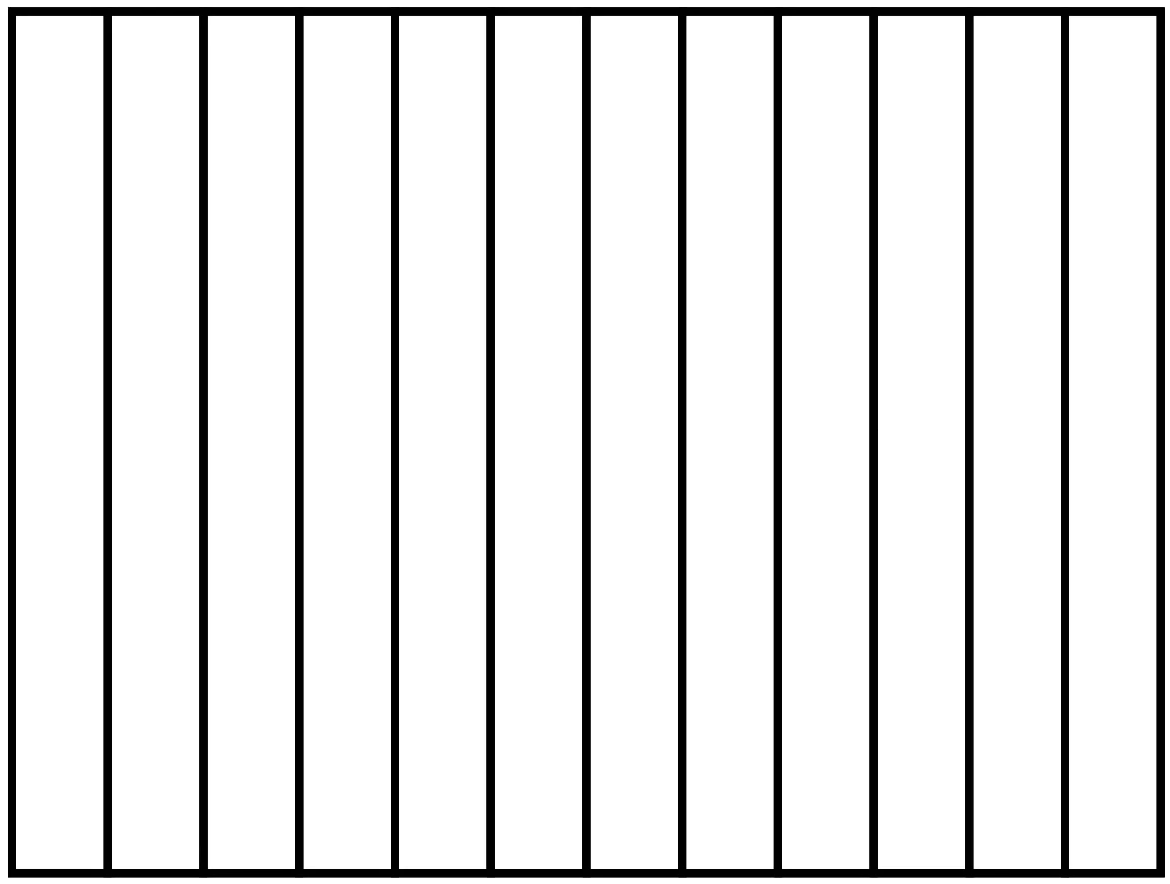
\includegraphics[width=10cm]{ss/grid-columnas.png}
\end{figure}
\begin{figure}[H]
    \centering
    \caption{Tamaño de un elemento según \textit{n} columnas de una fila del Grid}
    \label{fig:3}
    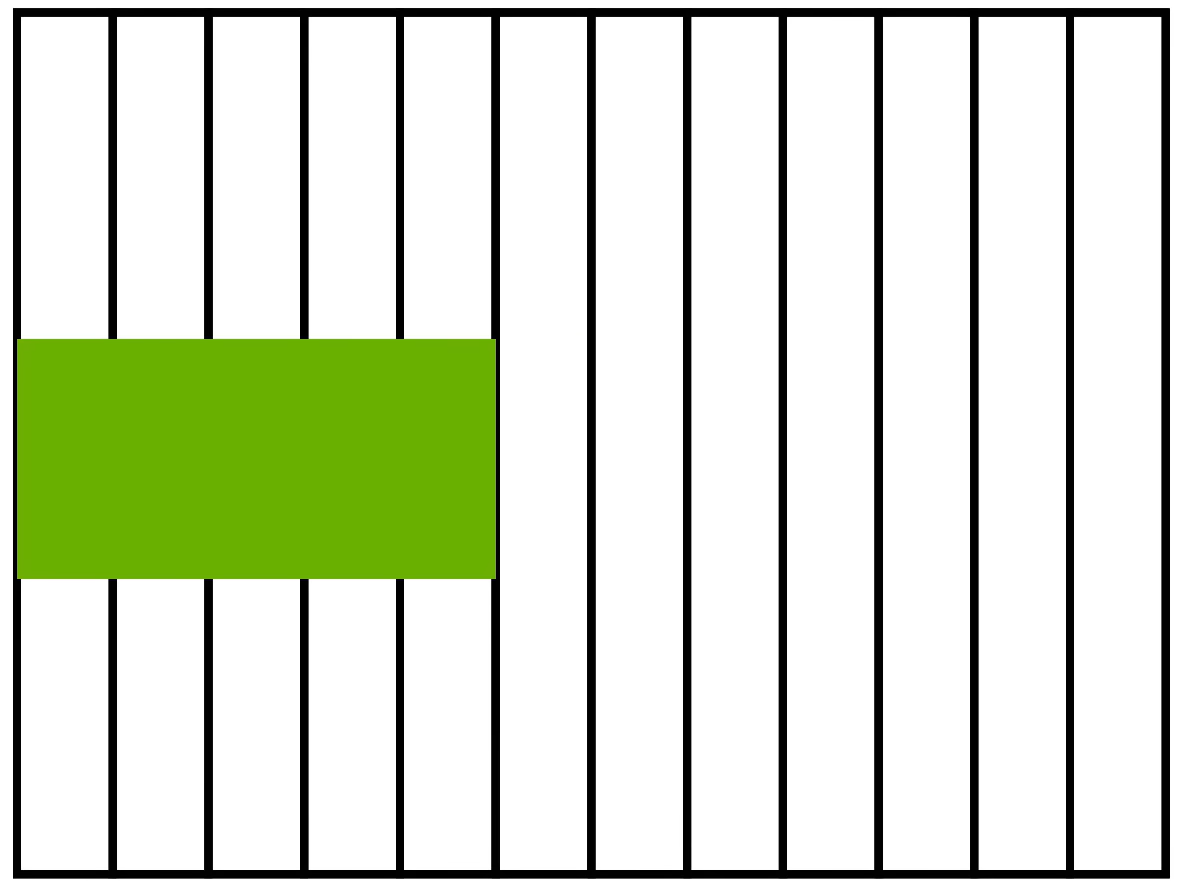
\includegraphics[width=10cm]{ss/grid-columnas-selected.png}
\end{figure}

Además, existen estilos predeterminados para distribuir y alinear los elementos de una página, como se ven en las Figuras \ref{fig:4}, \ref{fig:5} y \ref{fig:6}.
\begin{figure}[H]
    \centering
    \caption{Estilo de la Grid en panel uniforme}
    \label{fig:4}
    
\includegraphics[width=10cm]{ss/grid-estilo1.png}
\end{figure}
\begin{figure}[H]
    \centering
    \caption{Estilo de la Grid en filas no uniformes}
    \label{fig:5}
    
\includegraphics[width=10cm]{ss/grid-estilo2.png}
\end{figure}
\begin{figure}[H]
    \centering
    \caption{Estilo de la Grid en columnas no uniformes}
    \label{fig:6}
    
\includegraphics[width=10cm]{ss/grid-estilo3.png}
\end{figure}

Estos estilos se adaptan a las necesidades del desarrollador por mostrar el contenido de una u otra manera.


\subsubsection{Clases para la Grid}

Entonces, para utilizar la Grid dentro del desarrollo de una página web, es necesario recurrir a las clases de la Grid, las cuales están presentes en la Tabla \ref{tab:1}.
\begin{table}[H]
    \centering
    \caption{Ejemplos de clases de la Grid}
    \label{tab:1}
    \begin{tabular}{m{2cm} m{6cm} m{5cm}}
        \hline
        \textbf{Nombre} & \textbf{Definición} & \textbf{Dimensión} \\
        \hline
        .row        & \parbox{6cm}{Permite que un elemento HTML o Bootstrap se acomode como una fila, pudiendo abarcar cierta cantidad de secciones, columnas o un ancho de dicha fila. Es aquí donde entran las siguientes clases.} & \parbox{5cm}{El ancho de la ventana que lo visualiza o el contenedor que lo almacena} \\
        \hline
        .col        & \parbox{6cm}{Distribuye los elementos de una fila como columnas con un espacio definido o automático} & \parbox{5cm}{El ancho de la ventana que lo visualiza o el contenedor que lo almacena} \\
        \hline
        .col-xs     & \parbox{6cm}{\textit{xs} corresponde a \textbf{extra small}, es el tamaño más pequeño para una columna o elemento}        & $<576$px \\
        \hline
        .col-sm-    & \parbox{6cm}{\textit{sm} corresponde a \textbf{small}, esto define un tamaño pequeño para una columna o elemento}              & $>=576$px \\
        \hline
        .col-md-    & \parbox{6cm}{\textit{md} corresponde a \textbf{medium}, define un tamaño medio para una columna o elemento}               & $>=768$px \\
        \hline
        .col-lg-    & \parbox{6cm}{\textit{lg} corresponde a \textbf{large}, define un tamaño grande para una columna o elemento}                & $>=992$px \\
        \hline
        .col-xl-    & \parbox{6cm}{\textit{xl} corresponde a \textbf{extra large}, esto define un tamaño mayor a lg}                                  & $>=1200$px \\
        \hline
        .col-xxl-   & \parbox{6cm}{\textit{xxl} corresponde a \textbf{extra extra large}, es el tamaño más grande para una columna o elemento}   & $>=1400$px \\
        \hline
    \end{tabular}
\end{table}

Estas dimensiones representan el ancho de la ventana o pantalla del dispositivo donde se está visualizando la página, llamada también \textit{viewport}.


\subsubsection{Breakpoints}

Un punto de quiebre o \textit{breakpoint} es un ancho o dimensión determinado en el cual se puede cambiar la distribución, alineación o estilo de la página, es decir, si la resolución de la pantalla del dispositivo que está viendo la página web pasa de 700px a 465px, un breakpoint podrían ser los 500px, al bajar de esta resolución, los elementos se distribuyen de otra manera. Los breakpoints más comunes de Bootstrap 5 son las dimensiones en píxeles escritas en la tabla anterior, si utiliza una versión anterior, consulte los endpoints existentes en dicha versión.

Estos cambios de distribución o estilo de una página al pasar un breakpoint se puede apreciar en la Figura \ref{fig:7} y \ref{fig:8} respectivamente.
\begin{figure}[H]
    \centering
    \caption{Aspecto original previo a cambio por breakpoints en sitio real}
    \label{fig:7}
    
\includegraphics[height=10cm]{ss/breakpoints1.png}
\end{figure}
\begin{figure}[H]
    \centering
    \caption{Aspecto nuevo posterior al cambio por breakpoints en sitio real}
    \label{fig:8}
    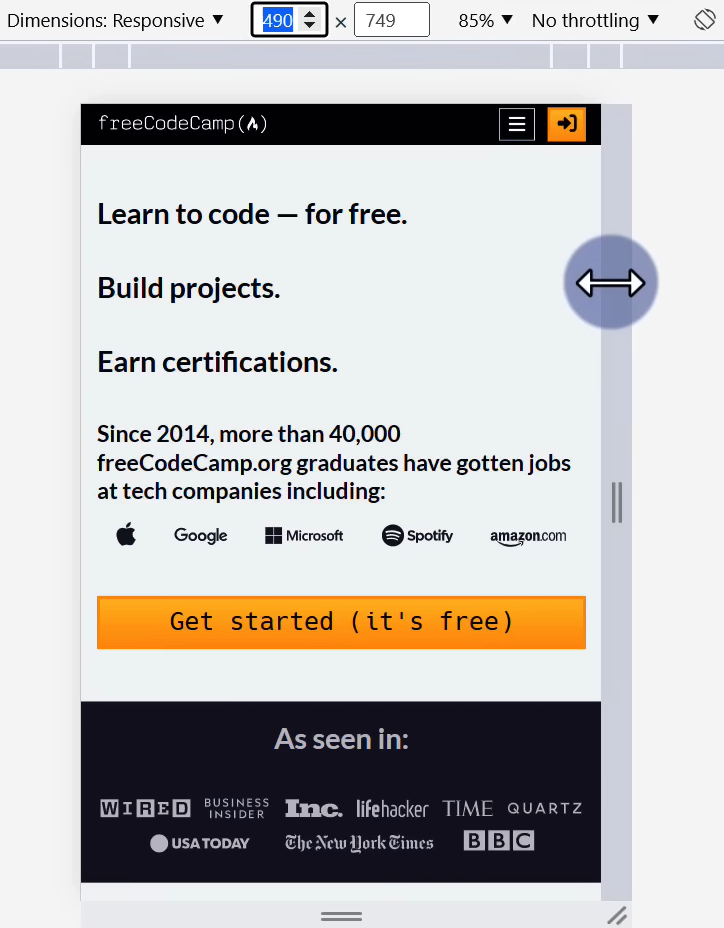
\includegraphics[height=10cm]{ss/breakpoints2.png}
\end{figure}


\subsubsection{Estructura}

Hablando más prácticamente de cómo será distribuido el contenido HTML en la Grid de Bootstrap, recordemos que podemos insertar la cantidad de filas que deseemos con la clase \textit{.row} y que cada fila estará seccionada por 12 columnas, con esto podemos darle el tamaño que deseemos a los elementos, siempre y cuando esté dentro de estas 12 columnas. Un ejemplo simple y visual es el siguiente.
\begin{lstlisting}
    <div class='container'>
        <div class='row'>
            <div class='col'></div>
            <div class='col'></div>
        </div>
        <div class='row'>
            <div class='col'></div>
            <div class='col'></div>
            <div class='col'></div>
        </div>
    </div>
\end{lstlisting}

Visualmente, tiene el aspecto de la Figura \ref{fig:9}.
\begin{figure}[H]
    \centering
    \caption{Uso de las clases de filas y columnas de Bootstrap}
    \label{fig:9}
    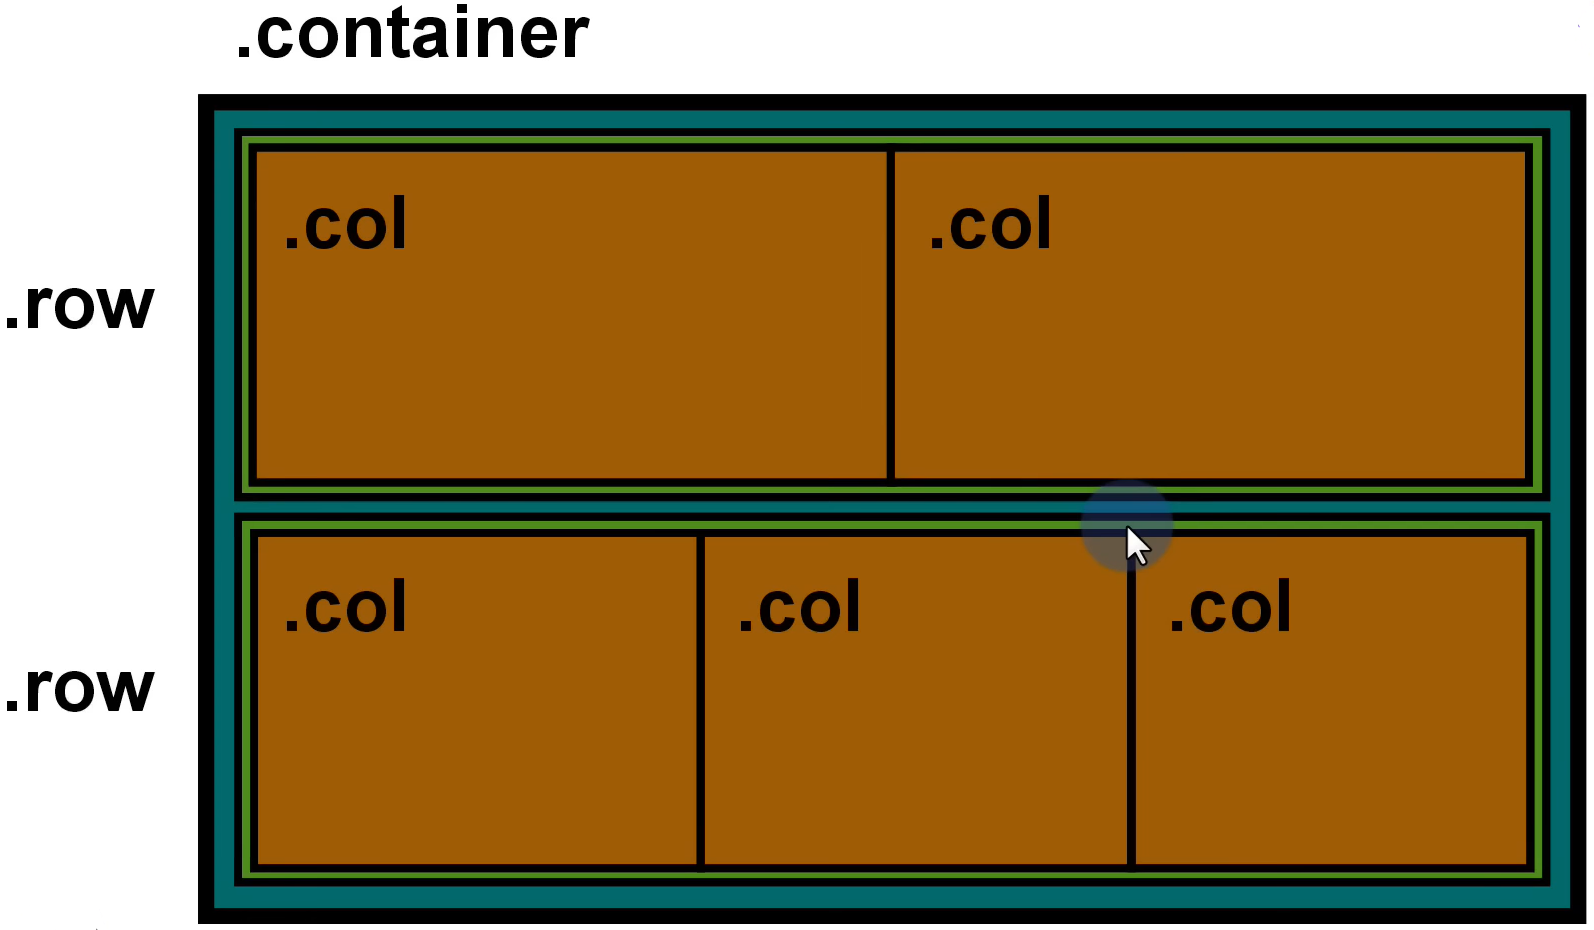
\includegraphics[width=10cm]{ss/grid-estructura.png}
\end{figure}

Donde el recuadro verde \textit{.container} almacena los recuadros cafés que representan los divs con las clases \textit{.row} y \textit{.col}, las líneas 2 a 5 representan la primer fila y dos recuadros dentro del recuadro verde, mientras que las líneas 5 a 10 representan la segunda fila. Podemos concluir que estas filas adoptan el ancho total de su contenedor y las columnas adoptan un ancho dependiendo del tamaño de su contenedor y de la cantidad de columnas que existe, de tal manera que su ancho final es uniforme entre el número de columnas.


\subsubsection{Contenedores}

En el ejemplo de la sección anterior, vimos que todas las filas y columnas utilizadas fueron contenidas dentro de un div \textit{.container}:
\begin{center}
    \textit{$<$div class='container'$>$$<$/div$>$}
\end{center}

Un contenedor Bootstrap es aquel que almacena todos los elementos HTML y Boostrap que serán distribuidos o utilizados por las filas y columnas del Grid de Boostrap, es decir, un contenedor que contendrá contenedores con las clases \textit{row} y \textit{col}.

Bootstrap maneja dos tipos de contenedores principales, los cuales son:
\begin{itemize}
    \item \textbf{.container}: esta clase crea un contenedor responsivo con un ancho máximo fijo que depende del ancho de la pantalla del dispositivo. Este contenedor no abarca la totalidad del ancho de pantalla, siempre deja un espacio en blanco o margen en las esquinas y se reduce en base a los breakpoints. La Figura \ref{fig:10} contiene un ejemplo visual de este contenedor.
    \item \textbf{.container-fluid}: esta clase crea un contenedor responsivo que cubre el 100\% del ancho de la ventana. La Figura \ref{fig:11} contiene un ejemplo visual de este contenedor.
\end{itemize}
\begin{figure}[H]
    \centering
    \caption{Aspecto original de la clase container}
    \label{fig:10}
    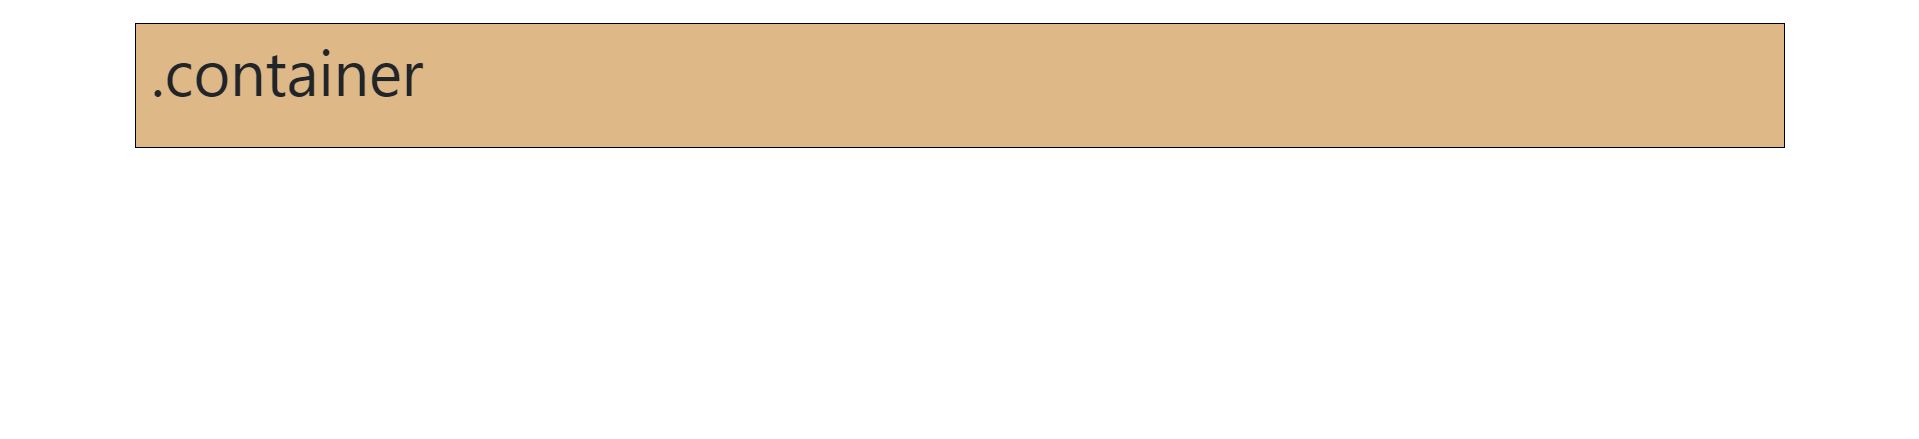
\includegraphics[width=10cm]{ss/container.png}
\end{figure}
\begin{figure}[H]
    \centering
    \caption{Aspecto original de la clase container-fluid}
    \label{fig:11}
    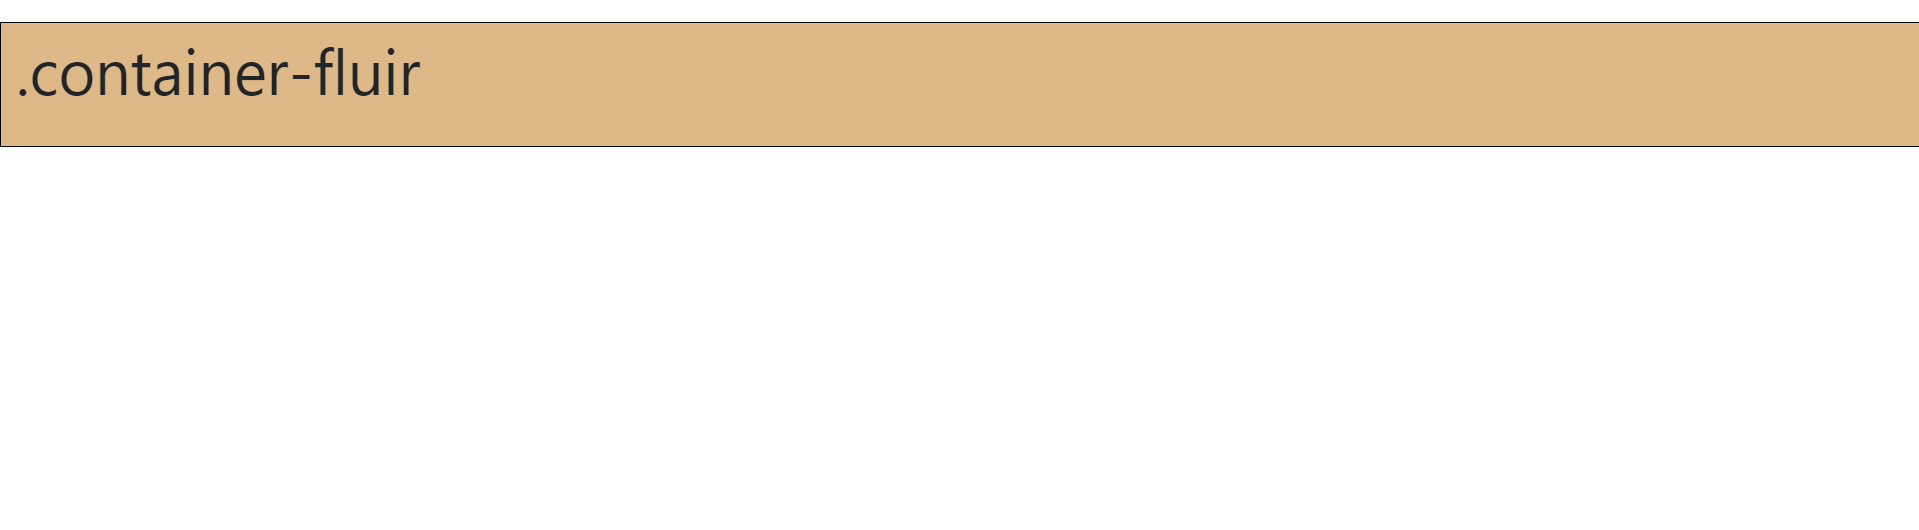
\includegraphics[width=10cm]{ss/container-fluid.png}
\end{figure}

La Figura \ref{fig:12} y \ref{fig:13} muestran el aspecto que toman las clases container y container-fluid después de reducir su tamaño.
\begin{figure}[H]
    \centering
    \caption{Nuevo aspecto de la clase container}
    \label{fig:12}
    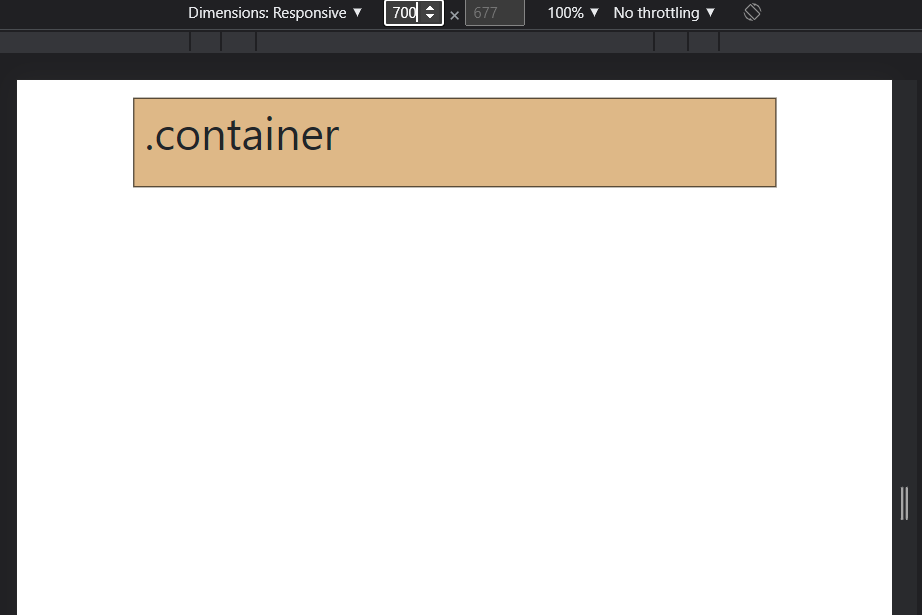
\includegraphics[width=10cm]{ss/container2.png}
\end{figure}
\begin{figure}[H]
    \centering
    \caption{Nuevo aspecto de la clase container-fluid}
    \label{fig:13}
    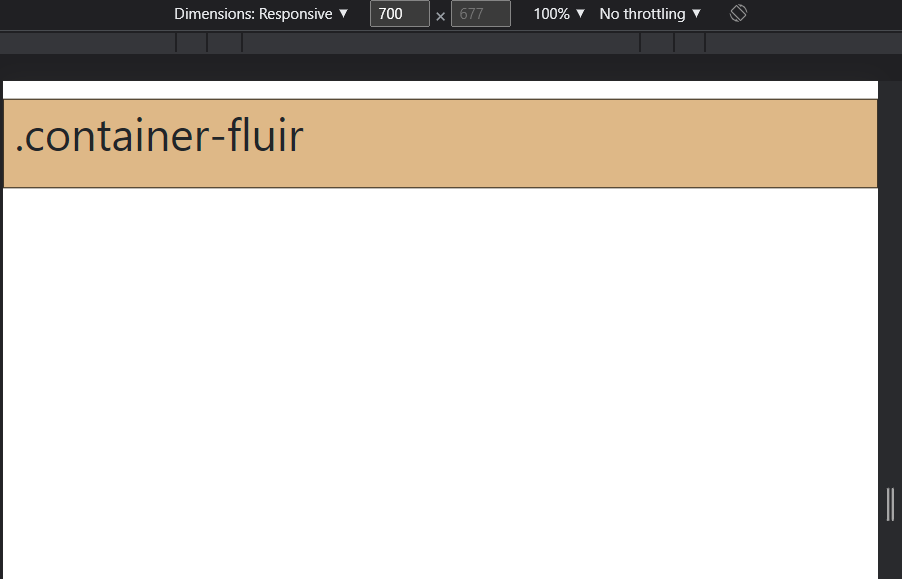
\includegraphics[width=10cm]{ss/container-fluid2.png}
\end{figure}


\subsubsection{Contenedores responsivos}

Estos contenedores cambian su tamaño cuando se llega a un breakpoint determinado, recordemos que los breakpoints básicos de Bootstrap están presentes en la Tabla 1, por lo que, al sobrepasar la cantidad de píxeles de algún breakpoint, el contenedor responsivo tomará un ancho fijo con respecto al tamaño de la pantalla, si menos pasa la cantidad de píxeles, el contenedor adopta el 100\% del ancho de la pantalla; dicho de otra manera, si sobre pasa el breakpoint, se comporta como la clase \textit{container}, si lo menos pasa, adopta el comportamiento de la clase \textit{container-fluid}. Los contenedores disponibles son:
\begin{itemize}
    \item \textbf{.container-sm}.
    \item \textbf{.container-md}.
    \item \textbf{.container-lg}.
    \item \textbf{.container-xl}.
    \item \textbf{.container-xxl}.
\end{itemize}

Veamos un ejemplo para comprender mejor estos contenedores.
\begin{lstlisting}
    <div class='container'>
        .container
    </div>
    <div class='container-fluid'>
        .container-fluid
    </div>
    <div class='container-lg'>
        .container-lg
    </div>
\end{lstlisting}

Añadimos las clases de los otros tipos de contenedores para que se puedan diferencias visualmente. La Figura \ref{fig:14} muestra como se ven los contenedores responsivos después del breakpoint, mientras que la Figura \ref{fig:15} muestra su aspecto después de menos pasar el breakpoint, como podemos concluir, primer se ve como un contenedor fijo y luego como uno fluido.
\begin{figure}[H]
    \centering
    \caption{Aspecto original de la clase container-lg}
    \label{fig:14}
    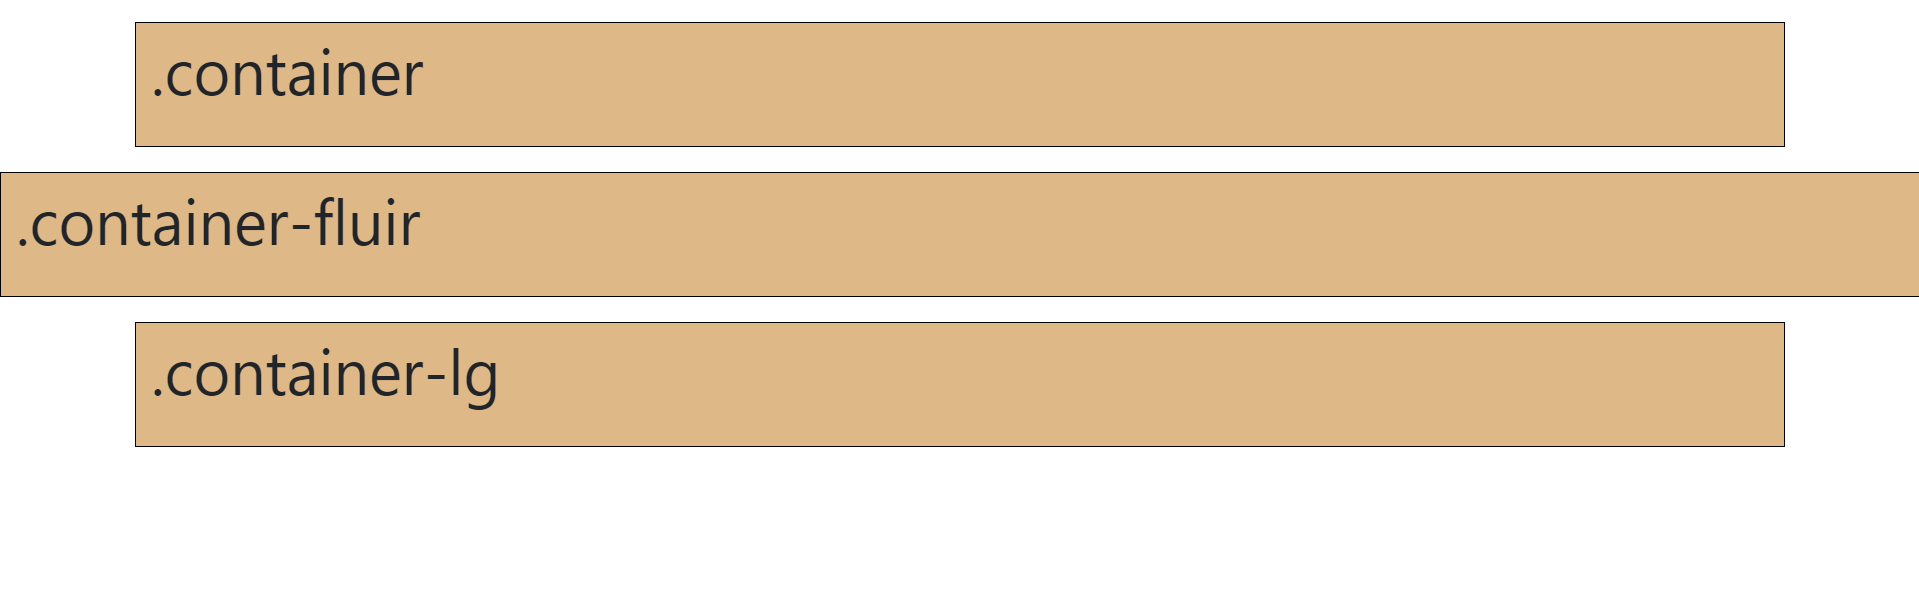
\includegraphics[width=10cm]{ss/container-responsive.png}
\end{figure}
\begin{figure}[H]
    \centering
    \caption{Nuevo aspecto de la clase container-lg}
    \label{fig:15}
    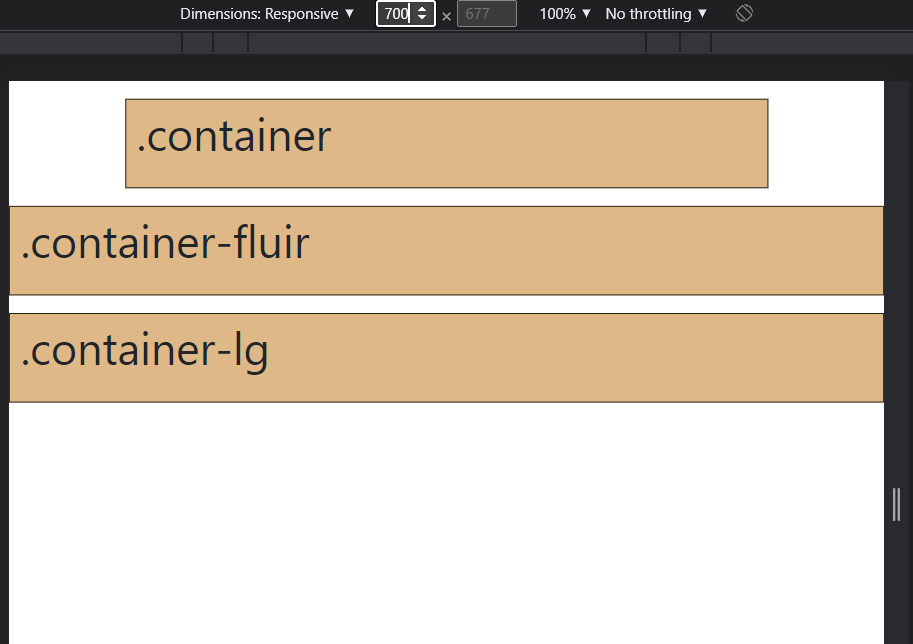
\includegraphics[width=10cm]{ss/container-responsive2.png}
\end{figure}

Este tipo de contenedores son efectivos cuando se pretende ajustar el contenido de la página a un tamaño específico de pantalla.


\subsubsection{Trabajando con las filas y columnas}

A las clases para la Grid se le puede agregar un valor entero positivo para que, menos pasar un breakpoint, adopte \textit{n} cantidad de columnas de la fila. La Figura \ref{fig:16} muestra lo anterior mencionado.
\begin{figure}[H]
    \centering
    \caption{Caption}
    \label{fig:16}
    \includegraphics[width=10cm]{ss/grid-tamaños.png}
\end{figure}

Note que, si el ancho de la página es menor a la dimensión establecida por el breakpoint \textit{sm}, el elemento con la clase \textit{col-sm-7} tomará un ancho de 7 columnas con respecto a las 12 de la fila en la que está situado, mientras que el elemento con la clase \textit{col-sm-5} adoptará 5 columnas. Debe fijarse que la suma de estos números enteros de como resultado 12, caso contrario colocará las columnas sobrantes en una nueva línea.

El siguiente ejemplo y la Figura \ref{fig:17} y \ref{fig:18} muestran un ejemplo sobre como utilizar estas filas y columnas con las clases para Grid y los contenedores.
\begin{lstlisting}
    <div class="container text-center">
        <div class="row">
            <div class="col-sm-4 col-lg-6 columna">
                .col-sm-4 .col-lg-6
            </div>
            <div class="col-sm-8 col-lg-6 columna">
                .col-sm-8 .col-lg-6
            </div>
        </div>
    </div>
\end{lstlisting}
\begin{figure}[H]
    \centering
    \caption{Aspecto original de los contenedores responsivos}
    \label{fig:17}
    
\includegraphics[width=\textwidth]{ss/row-cols1.png}
\end{figure}
\begin{figure}[H]
    \centering
    \caption{Nuevo aspecto de los contenedores responsivos}
    \label{fig:18}
    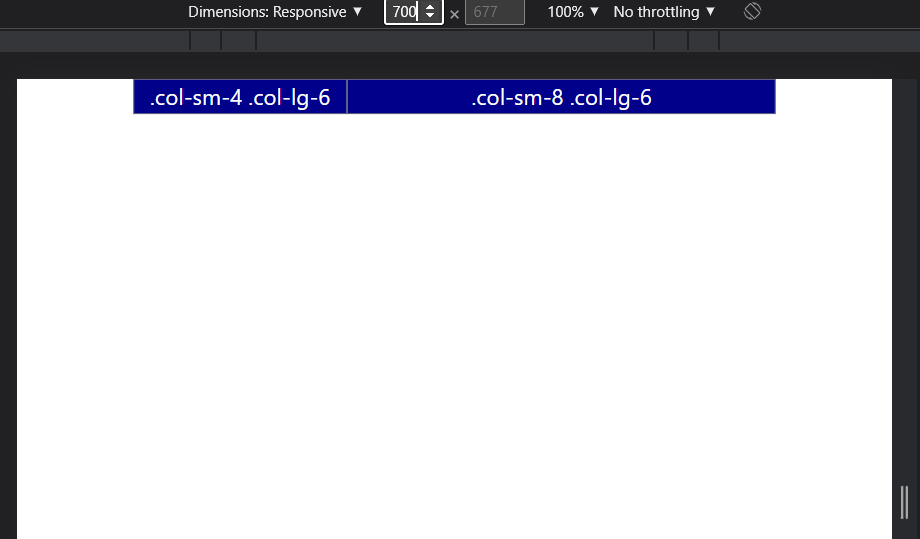
\includegraphics[width=10cm]{ss/row-cols2.png}
\end{figure}

La primer figura muestra como se ven las columnas cuando el ancho de la pantalla es grande, adopta el tamaño de la clase \textit{col-lg-6}, cuando este tamaño de pantalla es mejor a la resolución de \textit{lg}, adopta el tamaño de las clases \textit{col-sm-4} y \textit{col-sm-8} respectivamente. Estas clases son útiles para reajustar el contenido con base a los breakpoints.



\subsection{Componentes}

Los componentes de Bootstrap son etiquetas HTML reutilizables predeterminadas. Estos controles vienen con un estilo definido y pueden llegar a ser personalizados. Visite la \href{https://getbootstrap.com/docs/5.3/components/accordion/}{documentación oficial} de Bootstrap en su menú lateral izquierdo para consultar todos los componentes de Bootstrap disponibles, su visualización interactiva en el sitio y el código fuente para copiar e insertar en sus propios proyectos, simplemente siga las instrucciones de uso y modificación para aplicarlo a sus trabajos.


\subsection{Iconos}

Son recursos de imágenes gratuitos disponibles a usar en Bootstrap. Utilice este \href{https://icons.getbootstrap.com/}{\textcolor{cyan}{enlace}} para explorar todos los iconos disponibles y el pequeño tutorial para implementarlos en sus proyectos.


\subsection{Flexbox}

Flexbox es la abreviación de \textbf{CSS Flexible Box Layout}, vimos previamente que todos estos conceptos se enfocan en conseguir un diseño responsivo para el cambio de tamaño entre dispositivos que visualicen las páginas de nuestro sitio web, sin embargo, se puede utilizar Flexbox para que los elementos HTML o Bootstrap reajusten su tamaño, posición alineación dentro del contenedor que lo almacena de manera automática y uniforme.

Bootstrap utiliza clases que manipulan Flexbox de manera más sencilla y eficiente. La manera tradicional sería la siguiente.
\begin{lstlisting}
    <style>
        .cont {
            display: flex;
        }
    </style>
    
    <div class='cont'>
        Contenedor
    </div>
\end{lstlisting}

Mientras que con Bootstrap sería la siguiente.
\begin{lstlisting}
    <div class='d-flex'>
        Contenedor
    </div>
\end{lstlisting}

Los dos ejemplos anteriores realizan la misma función.


\subsubsection{Propiedades del Flexbox en Bootstrap}

La Tabla \ref{tab:2} muestra algunas de las propiedades básicas de Flexbox en Bootstrap.
\begin{table}[H]
    \centering
    \caption{Propiedades de Flexbox}
    \label{tab:2}
    \begin{tabular}{m{3cm} m{5cm} m{5cm}}
        \hline
        \textbf{Propiedad} & \textbf{Descripción} & \textbf{Clases equivalentes que hay en Bootstrap} \\
        \hline
        flex-direction  & \parbox{5cm}{Establece el eje principal del contenedor, la dirección en la cual se va a colocar los elementos dentro del contenedor. Los elementos se pueden alinear horizontal o verticalmente, regular o en reversa}         & --- \\
        \hline
        justify-content & \parbox{5cm}{\raggedright Esta define el cómo se tienen que distribuir los elementos en el eje principal}            & \parbox{5cm}{\raggedright.justify-content-start \\ .justify-content-end \\ .justify-content-center \\ .justify-content-between \\ .justify-content-around \\ .justify-content-wvenly \\ } \\
        \hline
        align-items     & \parbox{5cm}{\raggedright Define cómo se distribuyen los elementos en el eje perpendicular (o eje secundario) al eje principal}            & \parbox{5cm}{\raggedright.align-items-start \\ .align-items-end \\ .align-items-center \\ .align-items-baseline \\ .align-items-stretch} \\
        \hline
        flex-wrap       & \parbox{5cm}{\raggedright Determina si los elementos deben ser ajustados para que siempre estén en una misma línea o si se les permite distribuirse en varias líneas si es necesario}          & \parbox{5cm}{\raggedright.flex-nowrap \\ .flex-wrap \\ .flex-wrap-reverse} \\
        \hline
    \end{tabular}
\end{table}

En esta sección debe conocer el funcionamiento de Flexbox para visualizar y trabajar esta herramienta con Bootstrap, además de consultar la documentación para conocer cómo trabajar con el resto de propiedades disponibles.

% Fin del documento.
\end{document}